{
\begin{figure}[th]
\begin{center}
	\centerline{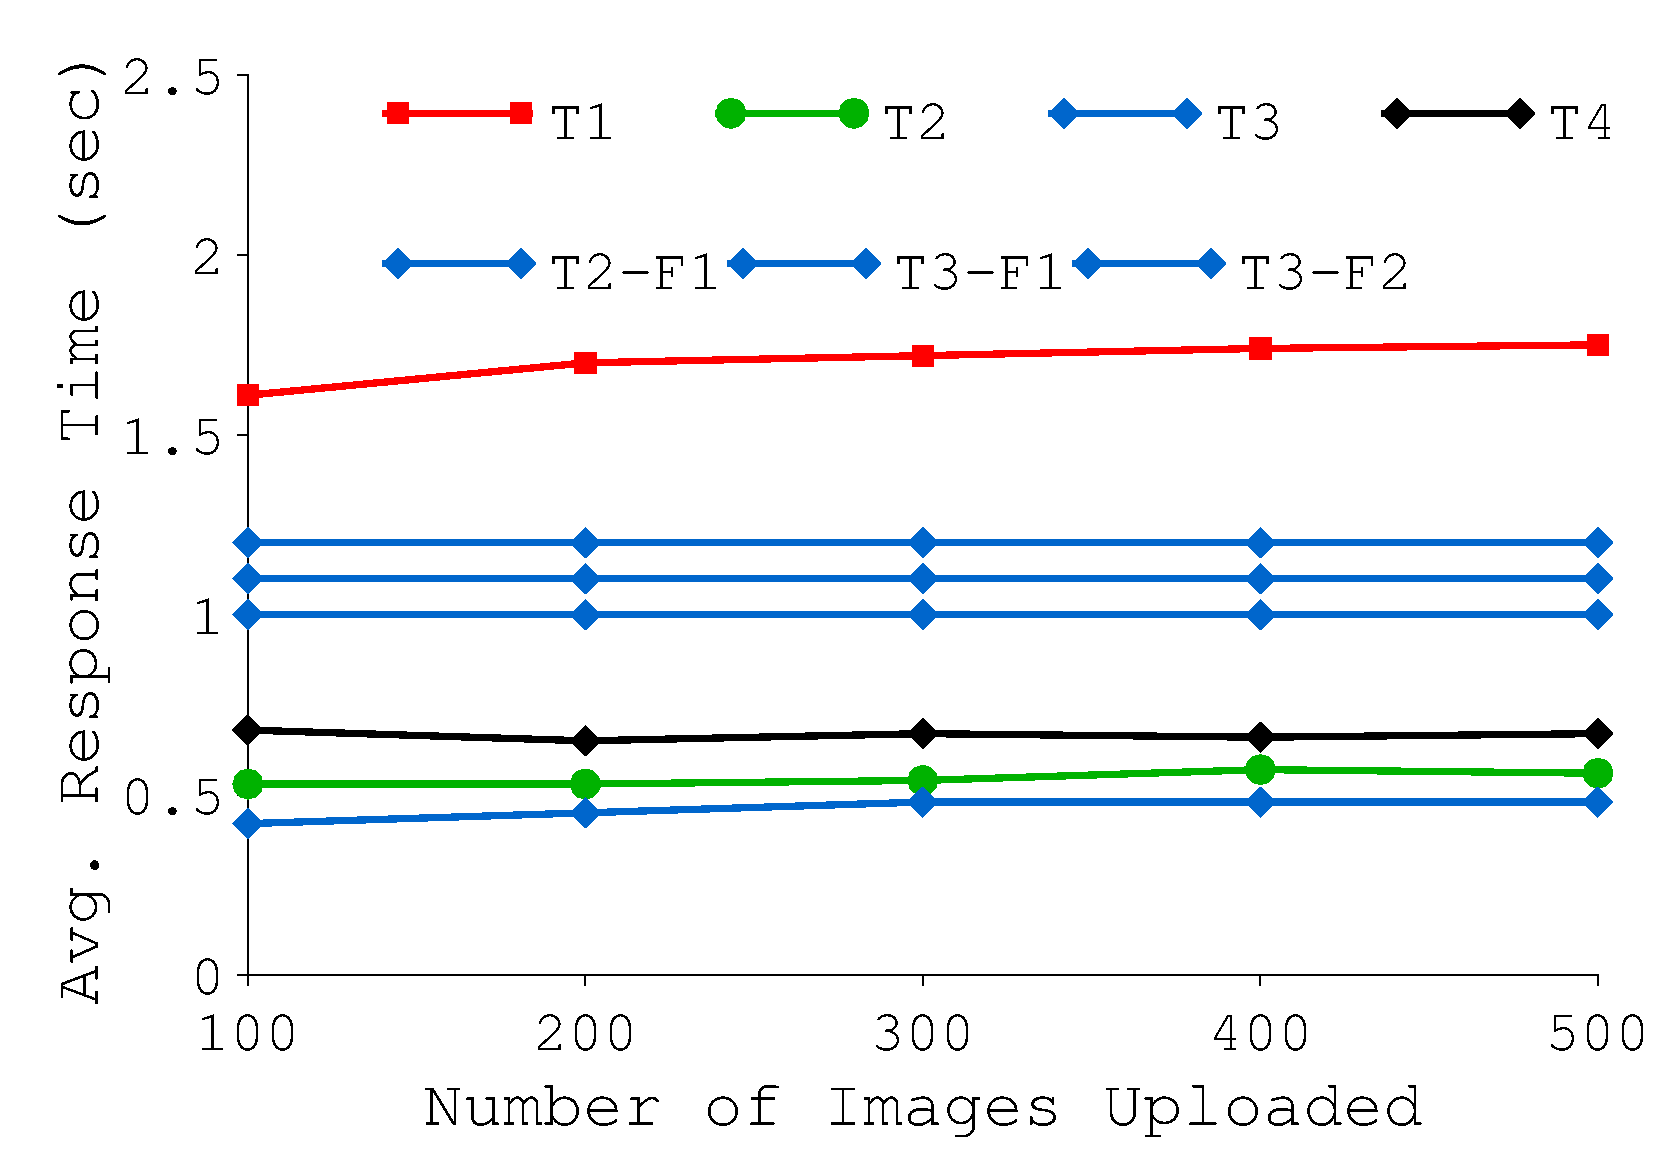
\includegraphics[width=2.5in]{Figures/g_plot_app.pdf}}
	\mycaption{fig-app}{Average Response Time With Different Computing and Failure Models.}
	{
		T1-T4 are performance without failure injected. Failure is injected 30 seconds
		after images have been uploaded. T2-F1 is the case where
		edge device failed during computation. T3-F1 is the case where the edge
		device received the uploaded images failed during computation. T3-F2 is
		the case where peer edge device failed. Application always re-send failed
		images to cloud.
	}
\end{center}
\end{figure}
}

